\documentclass[journal]{IEEEtran}
\usepackage[utf8]{inputenc}
\usepackage[official]{eurosym}
\usepackage{csquotes}
\usepackage{graphicx}
% \usepackage[caption=false, font=footnotesize]{subfig}
\graphicspath{ {./graphics/} }
\hyphenation{op-tical net-works semi-conduc-tor}

\begin{document}
\title{Internet Economics: A Survey}% <-this % stops a space

\author{Pablo~Carabana~Garcia,~\IEEEmembership{}%
        Benjamin~Fogg,~\IEEEmembership{}%
        and~David~Kirby,~\IEEEmembership{Student Member,~IEEE}%
\thanks{The authors are with the Department of Electrical and Computer Engineering, University of New Mexico, Albuquerque, NM 87131 USA (e-mail: pablocarabana@unm.edu; bfogg@unm.edu; davidkirby@unm.edu).}%
}

\maketitle
\begin{abstract}
Beginning in 1997, the field of Internet economics began to combine engineering principles with the study of economics to guide the development of national and international computer networks. Over the past decades, the field's boundaries have expanded thanks to the massive proliferation in consumer electronics, the new paradigms required by cellular networks, and new forms of media distribution. However, the emergence of modern streaming services, combined with a decrease in the number of available Internet service providers, has ignited a new debate centered around the topic of \enquote{net neutrality}. The original notions of a free and open Internet have been re-assessed in the light of these new technologies and their relationships to market forces. Net neutrality has pushed the study of Internet economics into the forefront and has forced engineers and technologist to not only consider how the future of the Internet will be built, but at what cost. Coupled with the COVID-19 pandemic, we see the future of Internet economics as at a crossroads where engineers and policy-makers must decide in which direction we shall proceed.
\end{abstract}
\begin{IEEEkeywords}
Network economics, Internet economics, net neutrality, content streaming, peer-to-peer networking, quality of experience (QoE), COVID-19, Coronvirus, pandemic.
\end{IEEEkeywords}

\section{Introduction}
\IEEEPARstart{T}{he} application of economic principles to the engineering of the Internet received its first formal treatment by McKnight and Bailey in 1997~ \cite{mcknightbailey97}. According to their work, the field is defined as \enquote{the study of the market for Internet services.} From this perspective, Internet economics has more in common traditional economic fields than it does the field of network engineering as McKnight and Bailey argued that even in 1997, at the burgeoning of the Dotcom era, \enquote{economic and policy issues must now be addressed to sustain the growth and expand the scope of the Internet.} It is our contention that this still holds true today and that the effects of the COVID-19 pandemic have further proven the fallacies in the Internet economics system and its failings to the typical rural American.

The fundamental topic of Internet economics, however, predates even McKnight and Bailey as in 1974 Leonard Kleinrock, the man who developed the mathematical theory of packet networks, considered the challenges of an \enquote{equitable charging and accounting scheme in such a mixed network system}~\cite{kleinrock74}. Today, the proliferation of multimedia delivered via Internet has reignited these considerations under the new banner of network neutrality \cite{faulhaber11}. The Internet was largely created as a small-scale solution to a relatively small-scale problem. However, even McKnight and Bailey reference \enquote{the convergence of [...] television, telephony, and computers,} along with the growing amounts of network traffic dedicated to \enquote{digital video, audio, and interactive multimedia}.

\subsection{Economics of Historical Networks}

Written before the turn of the millennium, McKnight and Bailey's paper could not have predicted the rise of media services like Napster, but by that time Usenet's distributed hosting structure had been used to establish \enquote{binary} newsgroups as a platform for piracy~\cite{seganusenet}. From there, it was a small step for Napster and LimeWire to leverage peer-to-peer data transfer beyond the newsgroup, with Napster gaining infamy by consuming up to 61\% of bandwidth on college campuses~\cite{napsterbandwidth}.

What could not have been predicted from knowledge of file-sharing on alt.binaries newsgroups was the rise of legitimate alternatives. Napster operated in its most recognizable form between 1999 and a United States federal injunction in July 2001, declaring bankruptcy in 2002. One year later, Apple extended their preexisting media player iTunes to include a music storefront, directly inspired by the ease with which Napster users could acquire new music~\cite{jobsandnapster}. This marked a turning point in the relationship of copyright media and the Internet.

%As license-holders and publishers rushed to the distribution opportunities offered by the Internet, the combination of more content and more customers demanding it began to burden network infrastructure. The authority an Internet service provider could exercise over not just their customers, but the content they were accessing, came into question. The proliferation of video streaming in the past ten years, coupled with the demand for higher-resolution media to stream, has resulted in bandwidth consumption at levels never before seen. The matter of network neutrality seeks to address

\subsection{Effects of COVID-19 on Internet Economics}
As the world is grappling with the effects of the COVID-19 pandemic, the Internet is being put through an unprecedented test as millions of people are being forced to stay at home, relying on the Internet as their sole method of work, school, entertainment, and source of necessities. This sudden surge in traffic as schools and workplaces cease all in-person operations have no doubt strained Internet services providers. And while there are reports of content distributors being urged to scale back their streaming quality~\cite{Forbes_Scaleback}, the Internet is scaling and adapting and, for the most part, is performing nicely. Indeed, there is much we can learn about the current state of Internet economics from this crisis and how we can improve it going forward.
\subsubsection{Survey of Current Internet Economics}
While the on-going crisis is a burden on us all, the Internet has taken a front-seat role as everyone must now rely on it to keep some semblance of normal life. Schools, work, and family life are now more dependant than ever on the backbone of the Internet keeping up with an ever-surging demand. It is therefore critical that Internet Service Providers (ISPs) keep customers connected during ever-demanding circumstances. This is why the Federal Communications Commission drafted the \enquote{Keep Americans Connected Pledge}~\cite{FCCpledge} by which broadband and telephone service providers will:
\begin{enumerate}
    \item not terminate service to any residential or small business customers because of their inability to pay their bills due to the disruptions caused by the coronavirus pandemic;
    \item waive any late fees that any residential or small business customers incur because of their economic circumstances related to the coronavirus pandemic; and
    \item open its Wi-Fi hotspots to any American who needs them.
\end{enumerate}
Through this voluntary pledge, ISPs are committing to securing the infrastructure of the vital Internet services needed to continue during this pandemic.
This commitment, however, can seem like an over-promise as many rural Americans are in areas that are under-served and lacking in adequate broadband capability. Indeed, the more pertinent concern is not whether the Internet can scale to cope with the rising demand, recent data shows that it can~\cite{IEEE_InternetCoping}, but whether it can be accessed at all. For upwards of 42 million rural Americans, broadband access is not an option~\cite{IEEE_broadbandRights}, which can mean the inability to work, attend school, or even communicate with loved ones. This \enquote{digital divide,} as FCC Commissioner Jessica Rosenworcel called it~\cite{FCC_Dissent}, is exposing the inequalities of the U.S. Internet infrastructure and presenting opportunities for where we can implement traditional economic policies to spur innovation and secure broadband for future crises.
\subsubsection{Vision for Post-Pandemic Internet Economics}
In MIT economist John Van Reenen's recent survey of American technological innovation~\cite{MIT_Economist}, we are given a thorough walkthrough of what Dr.\ Reenen considers the failures of American innovation. He covers the decline in American funding in Research and Design and discusses the economic methods by which we may correct this downward trend. We assert that his policy views are applicable to Internet economics, and given the current pandemic and inevitable future need to rebuild our economy, now would be the perfect opportunity to begin reforming America's Internet infrastructure in such a way as to promote tremendous growth.

\subsubsection{Related Work \& Contributions}
There have been various models that have laid out economic reasons for why most newer Internet technologies fail to reach viability. These include IPv6, differentiated service (DiffServ), and content delivery networks (CDN), where, of the three, only CDNs are being deployed at a reasonably effective rate~\cite{IPv6_Adoption}. These models claim that the causes for such lackluster roll-out are predominantly economic constraints rather than technological. Ye, Xie, and Lui in their conference paper for the 2018 IEEE International Conference on Network Protocols~\cite{IEEE_Deployability} presented a game-theoretic model comparing \enquote{the deployability of competing architectures} and implementation strategies that would be both profitable for ISPs and beneficial to end-users.

Our contributions are: to survey both the economic and game-theory models in light of the current pandemic and to assess rapid deployment and technological upgrades using economic policies from Reenen et al.

\subsection{Global View of Internet Economics}
As the Internet Association states in the study \enquote{Toward A Better Understanding Of Internet Economics}~\cite{IA_IE}, since the beginning of the computer age, scholars have struggled to understand the significance of these devices for society and the economy. By the 1960s the term \enquote{knowledge-based industry} started being used to describe this emerging sector and knowledge-producing occupations had surpassed other occupations in terms of the number of workers. By the 1970s, the \enquote{information economy,} was defined as those \enquote{specific industries and occupations whose primary function is to produce, process, or transmit economically valuable information.}

Recently, there has been increasing attention paid to the impact of the internet, and the emergence of an \enquote{internet economy.} Based on a series of communication standards that have been universally adopted, the internet has made it possible to transmit and to share information on an unprecedented scale. Initially, access to the internet was confined to fixed computers and terminals, but thanks to the popularity of smartphones and other wireless devices, which account for more than 3/4ths of all internet use, mobile access to the internet has become increasingly important.

In fact, the internet has become a \enquote{platform of platforms} that provides the basic infrastructure for a growing portion of all social and economic activity. Conceding that \enquote{the internet economy is an extensive and hard-to-capture sector,} the Internet Association has noted that it \enquote{is comprised of both unique industries and traditional activities conducted through new tools and platforms from the Internet.}

\section{System Model}

\subsection{Historical Networks and the Economy}
The earliest ancestor of the Internet and the first system to link computers over long distances was ARPANET, created under the US Department of Defense's Advanced Research Projects Agency. Founded by Dwight D. Eisenhower in 1957 as a response to the launch of the Soviet satellite Sputnik, ARPA's original goals were to expand science and technology beyond the immediate military applications required by the Cold War~\cite{eisenhowerarpa}. By creating ARPANET, the precedent for long-distance information exchange between networks was established. Services like NSFnet and Usenet followed not long after, establishing the first computer networks outside of government laboratories. Without federal defense research funding behind them, these newer services were forced to find alternative means, resulting in the first encounters of computer networking with free-market economic forces.

\subsubsection{ARPANET}
ARPANET was the first large-scale long-distance computer network, launched in 1969. By 1970, the first network protocol had been launched in the form of the Network Control Program.  It took another 14 years before packet switching would be implemented in the form of TCP/IP~\cite{arpanetswitch}. At its height it featured several satellite links and included both coasts of the United States, Hawaii, Germany, and Korea~\cite{meineldigitalcomms}. The project was formally discontinued in 1990, with NSFNet serving as its successor~\cite{nsfnet}.

ARPANET was conceived as a resource sharing system to reduce expenditures on computer hardware. Instead of purchasing computers for the various organizations within ARPA, it was determined than a system to network those that already existed would be a more efficient expenditure~\cite{quartermanarpa}.

Kleinrock's 1974 paper considered the problems of \enquote{large computer communication networks,} which he described as consisting of one thousand nodes or more. However, the computers discussed here are the time-sharing systems accessed via a terminal dialing into a mainframe. Notable about this paper is that it was written when ARPANET was still run on the Network Control Program, nearly ten years before the switch to the TCP/IP protocol in 1983. Concern for a network of one thousand nodes seems quaint with billions of devices on the modern Internet, but Kleinrock's primary concerns are flow control of messages and radio communications \cite{twobildevices}. Flow control was a much larger problem when ARPANET was using the Network Control Program, as the lack of packet switching did not yet allow for messages to be interrupted by other messages. As for the latter, if radio communications between computers are a precursor to wireless communication in general, then Kleinrock's ideas are not only relevant but essential concerns for the future of mobile computing.

Political ideas about competing economy left their mark on ARPANET in 1983, when the United States Department of Defense split the existing ARPANET infrastructure. Sixty-eight of one hundred and thirteen were removed from the ARPANET and placed into their own network, the MILNET, leaving ARPANET with only its civilian research nodes at universities. This split took place in the Reagan presidency, during the late years of the Cold War, and was explicitly enacted to restrict potential espionage~\cite{nytimesmilnet}.

ARPANET's status as a federal research project, coupled with its limited deployment to laboratories and federal universities, meant that it was a very exclusive and very expensive network. However, in 1986 the National Science Foundation constructed a successor to ARPANET in the form of NSFNET, another network intended for the sharing of research. By summer of that year, the creation of regional backbone network MIDnet in the Midwestern United States established the NSFNET as a precursor to the Internet.

\subsubsection{Early Internet}
In a rare case of the Internet affecting political and economic policy rather than the other way around, the 1992 work of an undergraduate student brought to light how the Internet's free exchange of information helped close out the Cold War. Hauben relays testimony from 1992, in the late days of the Soviet Union and East Germany, that attribute the breakup of Soviet authority to the Internet's free exchange of information \cite{haubenusenet98}. One teacher from Russia wrote him to explain: the personal computer's novelty, coupled with the waning government authority of the Gorbachev era, allowed digital communication to escape the ire of government censors. The Russian went on to explain that \enquote{It is practically the only way to communicate with the West[...] it was easier to access the PC in our institute than to get permission to use photocopy devices.} A student from Germany cited the Internet as an essential source after the 1989 Chernobyl disaster, as it was a rare news source not complicit in the Soviet government's cover-up work.

This student's work was conducted over the service known as Usenet, a distributed news publication and discussion network consisting of a wide selection of newsgroups. Dating all the way back to 1979 and dubbed \enquote{the Poor Man's ARPANET,} it offered a computer network to those without the six-figure capital and political connections necessary to join ARPANET. Instead, the only requirement was a Unix system and an autodial modem to contact other Usenet servers to exchange articles. All connections were made via piggybacking on existing links, including those used by ARPANET.

However, unlike the ARPANET links that it employed, Usenet was not immune to economic forces. Forces beyond technological progress again exerted pressure on the network in September 1993, a time that that came to be known as \enquote{Eternal September} \cite{eternalseptember}. This marked the date that America Online, the company that would become the largest Internet service provider within two years, offered Usenet service to its customers at no additional charge \cite{aolsize}. Usenet had seen influxes of new users in the past, with users unaccustomed to the particulars of \enquote{netiquette} arriving in time with college admissions in September. As new college students acquired access to computer systems for the first time, they were inducted into the customs and conventions of Usenet under the guidance of more experienced users, and gradually acclimated to the older ways. However, when AOL's multi-million subscriber count was unleashed upon Usenet all at once, the experienced users were massively outnumbered by the inexperienced, and so it became impossible to properly acculturate new arrivals. In January 1994, four months after AOL opened Usenet to millions, September 1993 was declared \enquote{the September that never ended} \cite{eternalseptember94}.

\subsubsection{World Wide Web}
The World Wide Web originated in 1989 with a proposal by Tim Berners-Lee, an engineer at CERN in Switzerland. By December, he had developed fundamental technologies such as the Hypertext Transfer Protocol, the Hypertext Markup Language, web server software, and the first web browser \cite{bernersleehttp}\cite{bernersleewebsoftware}. What distinguished this Web from the simpler Internet that preceded it was the usage of Uniform Resource Locators (URLs) organized under a Domain Name System that would resolve these URLs into the IP addresses of Web servers offering content. All of these transactions would be conducted over the TCP/IP protocol, which had seen its first large-scale adoption with ARPANET seven years prior. By January 1991, web servers began appearing outside of CERN, reaching the United States in September of the same year in the form of a catalog for the Stanford Linear Accelerator Center's online documents \cite{firstwebservers}.

Within five years of web server software reaching the public, Google Search launched. While not the first search engine for the World Wide Web-- that was 1993's W3Catalog-- the fact that more than one was deemed necessary indicated that the Web had spread beyond a single person's ability to maintain \cite{w3catalog}. Prior to W3Catalog's release in September of 1993, all webservers were manually catalogued by Berners-Lee \cite{bernersleewebcatalog}.

While the Internet had been established and the Web was flourishing, two barriers existed to the development of an Internet economy. The first was technological: Berners-Lee's web browser, the only web client in existence, had been developed on and for a NeXT workstation. Alternatives that ran on Unix's X Window System appeared by 1992, opening the Web to Unix and eventually Linux users. By August 1993, the Mosaic browser had versions for Unix, Macintosh, and Windows, opening the Web to major operating systems that still exist today \cite{mosaicbrowser}.

The second of these barriers was both cultural and hierarchical. In the 1990s, the NSF operated the backbone servers and connections of the Internet \cite{nsfbackbone}. Their word was effectively law, and so their principle that the Internet was for research rather than commerce enabled them to deny domain name registration to anyone seeking to use the Web for profit. This principle stood fast until 1995, and once the restriction was lifted, now-famous enterprises such as e-Bay (then known as AuctionWeb) and Amazon arrived before the year's end \cite{nsfcommerceorder}.

Less than ten years after the NSF opened the Internet to commercial interests, the world saw a boom and bust of Internet commerce in what came to be known as the dot-com bubble. After Netscape Communications patented SSL in March 1994 and packaged it with their Navigator browser, they had set themselves at the forefront of the economy of the Internet \cite{netscapessl}. Their entry into the stock market in August of that same year marked the beginning of the bubble, with founder Jim Clark's 20\% stake in the company worth five hundred million dollars by the end of the day \cite{netscapeipo} \cite{netscapebubble}. This marked the beginning of the bubble, an era where the returns on shares in Internet companies could average 88\% on the first day \cite{ljungvist02}. Even though brokerage K. Aufhauser \& Co. had been offering stock trading over the Internet since 1994, the five years of the dot-com boom were the first time the stock market had taken not

One of the more curious footnotes during the dot-coom boom was the virtual \enquote{beenz} currency. Offered by site beenz.com, this was not the first currency that could only be exchanged online -- that title belongs to the 1996 company E-gold, two years before the 1998 debut of beenz -- but it was a forerunner major currency that existed purely online \cite{virtualcurrencyhistory}. While E-gold was an Internet currency that could be exchanged for some amount of physical gold bullion, beenz had no such real-world counterpart. The proliferation of beenz prior to the dot-com bust and their closure 2001 proved that consumers were willing to place confidence in a currency with no material backing, showcasing new levels of consumer trust in items with no physical presence.

\subsection{Modern Network Economics - Fogg}
A new era of computer networking began with the release of filesharing software such as Napster in 1999 and LimeWire in 2000 \cite{napsterlimewiredates}. These were pieces of software that allowed users to publish their own files across the Internet for anyone to download through a peer-to-peer connection; Napster was focused on music, while LimeWire was used to distribute virtually everything. Both became infamous for their usage in the sharing of copyright files. Napster's time as a platform for piracy ended in 2001 after a legal battle with the Recording Industry Association of America, while LimeWire continued until a United States federal court injunction in 2010. While notable for their roles in shaping the legal relationship between the Internet and copyright, these services also brought filesharing out of Usenet obscurity and into the mainstream. The notion of Internet-based media distribution was relegated to these illicit forms until 2003, when Apple cooperated with major record labels to release their music via the iTunes store. Since then, media distribution has been one of the cornerstone usages of the Internet.

\subsubsection{Modern Content Distribution - Fogg}
As of 2015, data from Netflix at peak hours accounted for 36\% of all traffic on the Internet at that time \cite{spangler15}. This was only one year after offering the first 4K titles for streaming, when a 4K TV from Samsung cost one thousand dollars \cite{netflixadds4k}, \cite{tvprice}. Other networks like Hulu and Disney+ also offer 4K content as of 2016 and 2019, respectively \cite{hulu4k}, \cite{displus4k}. The rush to offer the highest resolution video content means there is consumer interest in the new video format, indirectly indicating a trend towards higher bandwidth consumption as more consumers switch to 4K content.

\subsection{Effects of COVID-19 on Internet Economics}
As millions of home-bound people turn to the Internet for their main lifeline to the outside world, there are concerns that the Internet is straining to keep up. David Rotman, in an article for the MIT Technology Review, wrote a scathing analysis stating that, \enquote{Those hoping the US could turn its dominant tech industry into a dynamo of innovation against the pandemic will be disappointed.} \cite{MIT_LackOfInnovation} There are reports of state unemployment websites crashing under the crippling demands \cite{IEEE_COBOL} as millions of Americans file for unemployment benefits. Outdated mainframes running code that is no longer taught in schools have caused these systems to crumble under the unexpected strain. One could pose the question why are these systems collapsing while sites that support much larger volumes of traffic such as Netflix and YouTube are able to handle exponentially more traffic without issue.\par
\begin{figure}[h]
    \centering
    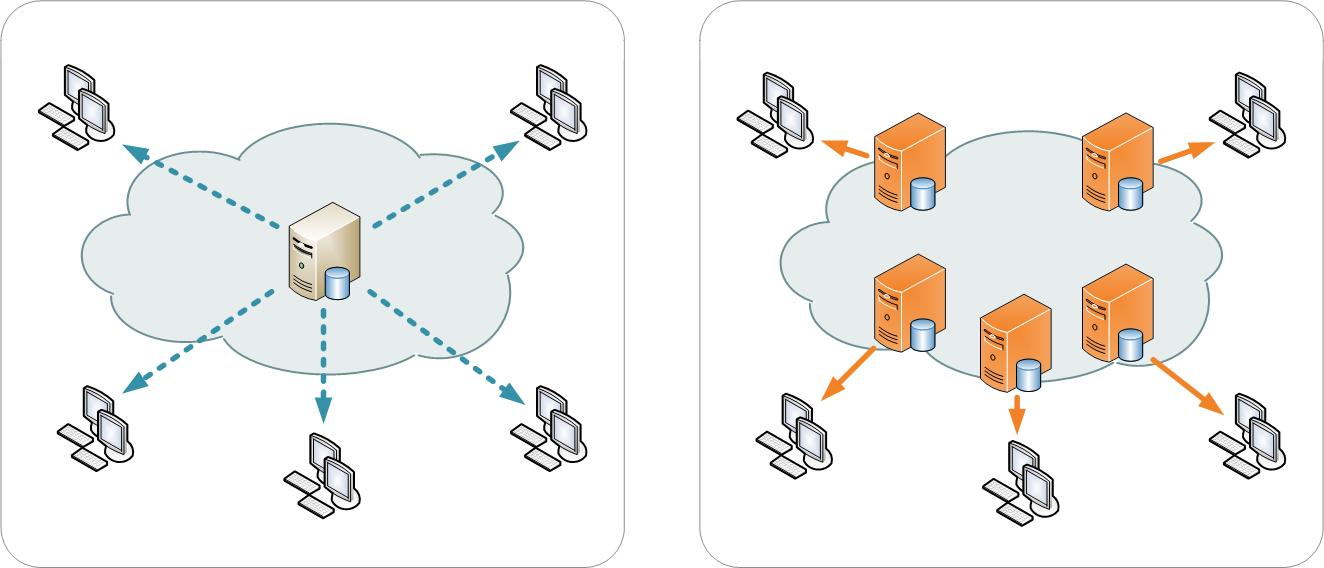
\includegraphics[width=0.45\textwidth]{CDN.png}
    \caption{Non-CDN vs. CDN. \cite{Graphic_CDN}}
    \label{fig:CDN}
\end{figure}
The answer lies in how the systems are designed and implemented. Content providers such as Netflix, Facebook, and YouTube are built to be deployed across a massive network of servers and databases. These content distribution networks (CDN) store and serve multiple copies of data from multiple geographically distributed nodes (see Fig. 1). This contrasts with the network of a typical state unemployment office which is hosted on a single, large \enquote{mega-server} and is susceptible to all of the faults that come with that design:
\begin{enumerate}
    \item single point of failure,
    \item point of network congestion,
    \item long path to distant clients, and
    \item multiple copies of the same data sent over outgoing link.
\end{enumerate}
This method is outdated and simply does not scale. There have been calls for retired programmers to help with the strain of this aging system, and while the middle of a pandemic is perhaps not the best time to upgrade a system such as this, it does signify the potential for future work.

It is not surprising then that Netflix and YouTube are handling the increase in traffic with ease. Network engineers have designed these systems to handle surges of this magnitude, albeit not during the middle of a weekday. However even these behemoths are not immune to the Coronavirus effect as European Union Commissioner Thierry Breton requested that they, along with Hulu and Disney+ throttle their systems \cite{Forbes_Scaleback} as a means to reduce Internet strains across Europe. For Netflix, this means maxing their streaming rate to standard definition, thereby cutting the network data by 25\%. It should be noted how little reducing the streaming quality impacts the overall data exchanged. This is due to the enormous amount of time, energy, and money that these streaming giants have spent perfecting their streaming and encoding algorithms. Netflix et al. are in the market of streaming to as many customers and as many devices as possible, and one can assume that their the Dynamic, Adaptive Streaming over HTTP (DASH) research has squeezed every bit out of the streaming process. Cheryl Idell, Chief Research Officer of WarnerMedia Entertainment has has announced that, while HBO is reporting a 20\% increase in TV viewing industry-wide \cite{HBO}, the Internet, given the circumstances, is showing incredible resiliency.

\subsubsection{Vision  for  Post-Pandemic  Internet  Economics}

As the globe begins to the emerge from the trenches of this pandemic, we are certainly going to be facing down an even tougher enemy. The effects of shutting down the global economy will undoubtedly be felt for at least the next decade.

This could however prove to be the reset that the global, and certainly U.S. economy has needed. Now, as millions of Americans find themselves without jobs and indeed companies are left in the ashes, what better time to start anew and to create the idyllic society that was once envisioned for 2020. There are myriad industries with which we could focus our attention. The Coronavirus has opened a glaring window into the faults and pitfalls of our society.

MIT economist John Van Reenen offered a path forward for technological innovation \cite{MIT_Economist} and we argue that these are no more prudent than for the Internet. Reenen lists three categories than propel the U.S. back into relevance on the Internet playing field:
\begin{enumerate}
    \item Tax incentives,
    \item direct government grants, and
    \item investments in skilled human capital.
\end{enumerate}

Reenen suggests that these three policies would drive research and design in the U.S. and argues that this should be government funded. With investments in these critical areas, we could see private sector innovation that would tremendous growth. When presented with the counter argument that corporations would simply relabel current projects to secure funding, Reenen supports his claim by suggesting, \enquote{A direct way to assess the success of the R\&D tax credit is to look at other outcomes such as patenting, productivity, or jobs.} As the economy is reeling from the effects of the COVID-19 pandemic, now would be the ideal time to stimulate the economy with fresh innovation, rather than blind bailouts. Millions of citizens are out of work with no hope of returning to work any times soon. We are suggesting a New Deal for the Internet Age, one where the highways and infrastructure built in the 1930s and 1940s is now mirrored in the highways and infrastructure of the 21st century Internet.

In addition to tax incentives, direct government grants would help public institutions such as universities and national laboratories also spur Internet innovations. In his analysis, Reenan posits that public grants often generate collaboration and direct benefit to private entities.

On top of the benefits to research and infrastructure, the benefits to skilled human capital would be immeasurable. If this pandemic has shown us anything, it is that the U.S. is severely lacking in the resources and desire to survive crises of this scale. While this pandemic will die down, there will inevitably be a new one, whether in the form of a virus such as COVID-19 or in the form of cataclysmic climate events, and the world and U.S. should be better prepared.

The New York Times, in an op-ed piece argued that for decades the U.S. has been failing to take the initiative, especially with regards to Internet and clean energy. This pandemic is, as FCC Commissioner Jessica Rosenworcel called it \cite{FCC_Dissent}, exposing the inequalities of the U.S. Internet infrastructure and presenting opportunities for where we can implement traditional economic policies to spur innovation and secure broadband for future crises. At least 42 million Americans cannot access suitable Internet, she argues. Matt Dunne, executive director of the Center on Rural Innovation, suggested in the New York Times piece that, \enquote{Building fiber infrastructure all across heartland America ensures that high-paying jobs can take place anywhere} and makes the country \enquote{more resilient to future pandemics and climate change-related weather events that require children and workers to stay home.} So many Americans are now Internet refugees without the hope of securing a job, school, or basic necessities. It is no wonder they are willing to risk their lives to get back to work. Imagine an alternative scenario where all Americans could, if they so choose, work from home, not have to commute, saving travel expenses because they can do so with a strong Internet backbone supporting them.

\subsection{Net Neutrality}
Network neutrality, more commonly known by its shortened title of net neutrality, is a movement originating from these debates over Internet service, monopoly, and bandwidth consumption. The term dates back to 2003, when it was coined by Columbia University law professor Tim Wu\cite{wu03}. He created the term as an Internet analogue to the older telecom notions of a common carrier. In the language of telecom, a common carrier is distinguished from a contract carrier by offering services impartially to the public, regardless of the person requesting the carrying (transport) or the item being carried.

A \enquote{neutral network}, according to Daniel J. Weitzner of MIT, has the following features \cite{weitzner06}:
\begin{enumerate}
    \item Non-discriminatory routing of packets
    \item User control and choice over service levels
    \item Ability to create and use new services and protocols without prior approval of network operators, and
    \item Non-discriminatory peering of backbone networks.
\end{enumerate}

In less technical and more popular terms, a neutral network is one that does not distinguish between any packet being transported and any other packet \cite{wirednetneutrality}. Network neutrality advocates fear that classifying packets will allows ISPs to lock or limit customer access to network services. This ties into the second point of Weitzner's definition: user control and choice over service levels. Once an ISP knows that one service or another is consuming more bandwidth, it would have the power to restrict movement of that service's packets on its networks. This may come in the form of a paywall, requiring users interested in the service to pay an additional fee to access it, or ban its access outright. This has already been seen in Therefore, according to Weitzner, to be \enquote{pro-neutrality} is to oppose the enactment of these restrictions and support legislation forbidding Internet service providers from ever employing them. \cite{weitzner07}.

Considering that Comcast, a major Internet service provider, also owns a major media company in the form of NBC Universal, fears of content micromanagement by Internet service providers have a basis in reality. While Comcast does not currently operate their own content distribution services, their 2018 acquisition of streaming service Xumo as \enquote{an independent business} has recently changed this dynamic \cite{xumoacquisition}. By operating as an Internet service provider, news source, and content distributor, Comcast has the \emph{theoretical} power to produce news via the NBC network, distribute it, and prevent users on their network from Clearly, such an ideological monopoly runs contrary to the scholarly intentions of early computer networks, and so network neutrality policy exists to provide preventative oversight.

The difficulties of network neutrality result from the need to balance ideology with reality. As discussed, Netflix consumes a disproportionate amount of all network bandwidth. However, with network neutrality policies in effect, Internet service providers are unable to reconcile the costs of hosting a service with their network, and so are forced to absorb the loss.

Analyzing the current situation of the debate about net neutrality worldwide \cite{COIT}, it can be seen that it has become more relevant in the United States than in Europe. In the United States, the debate has spread to almost every level with competencies in the regulation of telecommunications. The FCC (Federal Communications Commission) has taken a relatively extreme stance regarding free access to Internet content. In 2005, it established the main basic principles for Internet access, which are the right to access legal content and applications, to access the devices of your choice and to obtain information of interest about your service plan. Later, in 2010, transparency, non-blocking and non-discrimination were added to the already established principles. However, all of these principles were later rejected in 2011 by the Republican-controlled House of Representatives. Meanwhile, in Europe, a more neutral position has been preferred. Nevertheless, many of the final decisions regarding this issue have been taken based on some of the premises defended in the United States. The European Commission leads the debate on net neutrality in Europe. Until 2012, \enquote{active waiting} was the European Commission’s strategy. It analyzed and collected information and intensively monitored the operator behaviors. Through different directives, it has guaranteed and promoted access to content, as well as the users’ ability to access and distribute information through the Internet, promoting transparency and competition among different markets.

Only a few countries have delved into specific regulatory frameworks for this issue. There are several topics of debate regarding net neutrality, and the existence of different points of view is what is making it difficult to reach a solution is approved by the majority.

Transparency is an important aspect to take into account when dealing with this debate. The vast majority of organizations stipulate that the end user should be able to obtain information about the characteristics of the services that are being offered and to choose the provider that best suits his needs. For that information to be useful, it must be accessible, understandable, meaningful, accurate and proportionate. Transparency is a basic principle that has been endorsed by all actors involved in the net neutrality debate, and must be achieved for all products and services. The user has the right to know how operators manage traffic and under what circumstances. For the Internet to work correctly and smoothly, it is necessary for operators to apply reasonable and transparent traffic management. Although transparency does not discriminate between different technologies, it is a stronger need in certain technologies such as mobile given its characteristics and limitations.

However alone, is not fully effective and does not lead to a clear solution to the Internet neutrality debate. It is necessary to include other factors such as the quality of the service offered and the capacity of the operators to manage the traffic they handle. The parameters of the quality of service, QoS, are those that allow implementing the efficiency of Internet access. However, what is important for the user is the quality of experience, QoE, which is the quality that he perceives in the use of the service. Internet providers face the problem of increasing traffic on their networks, and to try to improve QoS or QoE, they must manage that traffic as efficiently as possible.

This leads to the key point of the debate, the possibility of managing Internet traffic. The evolution of the applications and the requirements associated with them (mainly the delay) do not always need the same type of network features. For this reason, the need to manage traffic adapting it to its characteristics becomes visible. The Internet has been developed under the principle of non-discrimination in traffic with the best effort model. However, QoS and different priority levels have always been seen as part of the Internet protocol. There are traffic decongestion techniques and tools that, although they may represent a rejection of the basic principles of the open Internet, in many cases they are used to maintain the security and integrity of the network or to avoid congestion. Some examples of those techniques are packet removal techniques, traffic prioritization, packet filtering, routing techniques and Deep Packet Inspection (which is used to block peer to peer traffic). The type of use given to these techniques is what will determine whether it has a positive or negative impact towards free Internet access. If, in order to manage congestion, traffic is prioritized or restricted in a non-discriminatory manner, no principle of network neutrality is violated. However, in order to allow discrimination, there must be a high degree of transparency.

Another topic of interest in this debate is the interconnection of systems, or IP interconnection using peering or transit techniques. Operators acting as Internet access service providers, ISPs, sell broadband access and Internet connectivity. Usually, they make wholesale interconnection agreements with other ISPs for the exchange of traffic. In general, all interconnection relations have been developed under the best effort model without causing any problems. However, the risk of an inappropriate way of using it can make this situation change, leading to the necessity of including wholesale IP interconnection relations within the scope of network neutrality. On the other hand, IP interconnection has been progressing, adapting to market developments, changes in technology and the necessary investments, and this has been possible without the need for any type of ex-ante regulation. Due to the exponential growth that Internet traffic has suffered, large content and application providers have negotiated directly with these ISPs. This has had a positive impact on aspects such as Quality of Service. As user demand has become more sophisticated, the evolution of CDNs (Content Delivery Networks) has done so too. More and more content providers are processing their own traffic, generating their own CDN network and reaching agreements directly with the operators. As a result, they may be considered to be violating the principle of best effort.

The different positions on network neutrality are polarized. While some defend the current situation with minimal intervention in regulation, others define a framework relationship where the principles that should govern the relationships between the parties involved in the Internet value chain are defined. No agreement has been reached yet.

The Internet ecosystem consists of the agents involved in the value chain, such as manufacturers and suppliers of devices, software, services, applications and operators. Until now, the debate on net neutrality has been focused only on operators, but it is necessary to analyze all the parts in order to reach some kind of solution. Past researches conducted by BEREC and the European Commission on the management of operators in Internet access revealed that operators generally did not prioritize or block traffic. On the other hand, if some practices of other agents in the Internet value chain were analyzed, it could be seen that in some cases traffic was prioritized. In these cases, access to certain content is restricted or traffic is prioritized to the desired content. In cases where the principles of transparency are not used or traffic management is exceeded, it is possible that it is being limited to a certain extent to the end user, and even limiting the technological innovation that the Internet allows.

Therefore, in order to obtain a global vision of the situation and to assess all the points of view in this debate, it is necessary to take into account all the agents and their different practices, to see what is correct and what is not correct according to the neutral point of view that offers network neutrality.

Network regulation in Europe is governed by the Body of European Regulators for Electronics Communications (BEREC) \cite{BEREC}. BEREC has developed the \enquote{Guidelines on the Implementation by National Regulators of European Net Neutrality Rules}, designed to provide guidance on the obligations of NRAs to service providers. These Guidelines deal with the safeguarding of open internet access, the required transparency measures for ensuring open internet access, supervision of network usage, and enforcement and penalties for violations of the previous guidelines.

More specifically, BEREC's guidelines state the obligations to closely monitor and ensure compliance with the rules to safeguard equal and non-discriminatory treatment of traffic in the provision of internet access services and related end-users rights. They constitute recommendations to NRAs in order to promote consistent application of the Regulation, providing stakeholders a certainty that the regulations are being followed.

\subsubsection{Internet Economics}
The Digital Assembly held in 2018 in Sofia (Bulgaria) \cite{DA_DE} analysed the data economy and the next generation Internet aspects, in the context of a common European data space. They concluded that the data-driven economy is increasing competitiveness, innovation and business opportunities at a world-wide scale, and rising global data flows have boosted world GDP by more than 10\% \cite{MGI_AA} and the value of the EU data economy was more than \euro{300} billion in 2016, representing more than 1.99\% percent of the EU GDP \cite{IDC_EDM} \cite{IDC_PD}.

This revolves around the generation of value out of data that, under favourable policy regulations, legislative conditions and investments in ICT, might increase the value of the European data economy to \euro{739} billion by 2020, representing 4\% of the overall EU GDP \cite{EC_EDS}. The potential that data holds becomes even larger when public sector information is combined with privately held data, which constitutes another pillar in the EU data economy.

The total investment in European telecom networks was \euro{48.6}bn in 2018 \cite{ETNO_SDC}, with ETNO companies deploying 70.5\% of the total network investment in Europe (\euro{34.4}bn, fixed and mobile). ETNO companies have the highest proportion of revenues dedicated to investment among global peers in US, Japan and South-Korea. However, investment per capita in Europe remains lower than those peers, with Europe investing around \euro{89} per person, as opposed to peers’ average at \euro{177} per person. European markets remain fragmented, with 47 main MNOs in Europe, as opposed to 7 in the USA, and 3 in South-Korea and Japan respectively.

ETNO has recently published the study entitled \enquote{Delivering Consumer Value in Digital Times} \cite{ETNO_DCV}, where is stated that investments around customer innovation are paying off. Consumers in European countries report a positive perception of the sector, and feel increasingly satisfied by what they get, and telecom operators rank highly on important issues such as privacy, data protection and consumer trust. European operators feature among the highest in international accountability indexes – demonstrating the attention they are putting on data governance and transparency related practices. As a result, customer engagement is improving as operators have adopted a customer-centred approach.

The sector has improved trust and is promoting fairness and value, and has seen record levels of investment both in terms of network and services for consumers, and operators are taking this further still by investing in the networks of the future which will provide a whole range of new innovative services and industries. As a result, consumers benefit from faster speeds and availability of innovative services, and operators are set to deliver dramatically increased value to consumers by enabling services they use for the most.

Having a comprehensive and objective view of how the sector is evolving is of key importance to pursue sound and evidence-based future policy-making. Whereas room for improvement always remains, especially in highly evolving sectors, we can see the progress being made. Prices are falling and consumers are getting more value from the services they use. Compared to regulated utilities (such as electricity, water, and gas) the sector is offering lower prices, more choice, and better customer satisfaction, as consumers benefit from an increasing range of tariffs and services.\cite{ETNO_DCV}

An important point to consistently compare the so called \enquote{Internet Intensity} among the nations of the OECD is to establish standardized indexes to measure the depth and reach of the Internet in commerce and society among, looking at the three measures of Internet activity \cite{BCG_CK}:
\begin{enumerate}
    \item Enablement: how well built is the infrastructure and how available is Access?
    \item Expenditure: how much money are consumers and businesses spending online e-commerce and online advertising?
    \item Engagement: how actively are businesses, governments and consumers embracing the Internet?
\end{enumerate}

\subsubsection{The European approach to Internet Economics and Net Neutrality}
According to the European Telecommunications Network Operators' Association (ETNO) \cite{ETNO_DCV}, Europe has initiated a transformation path towards a Gigabit Society, aiming to have every European citizen benefit from full digital environment by 2025. A Gigabit Society would allow citizens access to new, innovative services and products but requires cutting-edge connectivity. The Gigabit Society targets the attainment of networks speeds significantly above 100 Mbps for all the European consumers and 1 Gbps for public institutions, mayor transport hubs, and digitally intensive businesses.

\section{Conclusion}
Since 1997, Internet economics have settled into an uneasy balance between users and service providers. Users desire their fill of content at ever-increasing resolutions, while ISPs work to recoup the losses. Network neutrality stands between these two stances, preventing interference for particular content but preventing service providers from targeting any hosted service regardless of their usage. These changes have altered the field as it was originally set forth by McKnight and Bailey, though the need remains for the market and the Internet to adapt to one another.

Stories of the COVID-19 pandemic will be told for generations; about how the economy was crippled and millions lost their lives and livelihoods. If we do not take this crisis with a grain of salt and heed some lessons from it, then it will have been a wasted opportunity. Internet economics is not an easy balancing act with which to deal. As we have presented here though, there are many opportunities that we can take advantage of to be better prepared for the next event. As Li, Xie, and Lui have shown \cite{IEEE_Deployability}, the issue is not with technology, the solutions are there, the drawbacks are in the implementation. The economic policies are there too, we need only to implement them as well.

%\begin{table}[!t]
%\renewcommand{\arraystretch}{1.3}
%\extrarowheight
%\caption{An Example of a Table}
%\label{table_example}
%\centering
%\begin{tabular}{|c||c|}
%\hline
%One & Two\\
%\hline
%Three & Four\\
%\hline
%\end{tabular}
%\end{table}

% use section* for acknowledgment
\section*{Acknowledgment}
The authors would like to thank the University of New Mexico for the generous access to research material, as well as the opportunity to explore the past and present of the Internet.

\begin{thebibliography}{6}

\bibliographystyle{ieee}

 \bibitem{mcknightbailey97}
 L.~W. McKnight and J.~P. Bailey, \enquote{An Introduction to Internet Economics}, \emph{The Journal of Electronic Publishing}, vol. 1, no. 1 \& 2,\hskip 1em plus
  0.5em minus 0.4em\relax Jan. 1997

 \bibitem{seganusenet}
 S.~Segan, \enquote{R.I.P Usenet: 1980-2000}, \emph{pcmag.com}, July 2008. [online] [Accessed: Apr. 10, 2020].

 \bibitem{napsterbandwidth}
 P.~Fusco, \enquote{Network admins—especially at universities—are tearing their hair out[...]}, \emph{isp-planet.com}, March 2000. [online] [Accessed via Internet Archive: Apr. 10, 2020].

 \bibitem{jobsandnapster}
 S.~Knopper, \enquote{iTunes' 10th Anniversary: How Steve Jobs Turned the Industry Upside Down}, \emph{Rolling Stone}, Apr. 2013. [online] [Accessed Apr. 10, 2020].

 \bibitem{kleinrock74}
 L. Kleinrock, \enquote{Research Areas in Computer Communication}, \emph{Computer Communication Review}, vol. 4, no. 3, July 1974.

 \bibitem{eisenhowerarpa}
 Dwight D.~Eisenhower Memorial Commission, \enquote{Dwight D. Eisenhower and Science \& Technology}, \emph{eisenhowermemorial.org}, November 2008.

 \bibitem{quartermanarpa}
 J.~S.~Quarterman, \enquote{The Global Matrix of Minds}, \emph{Global Networks: Computers and International Communication}, 1993.

 \bibitem{meineldigitalcomms}
 C.~Meinel, H.~Sack, \enquote{Digital Communication: Communication, Multimedia, Security}, February 2014. p. 75.

 \bibitem{arpanetswitch}
 J.~Powers, \enquote{January 1, 1983: ARPANET Switches TCP/IP}, \emph{dayintechhistory.com}, January 2014. [online] [Accessed: Apr. 7, 2020]

 \bibitem{nytimesmilnet}
 W.~J.~Broad, \enquote{Global Computer Network Split as Safeguard}, \emph{The New York Times}, October 5, 1983.

 \bibitem{haubenarpanet}
 M.~Hauben, \enquote{History of ARPANET}, \emph{Site de l'Instituto Superior de Engenharia do Porto}, 2007.

 \bibitem{nsfnet}
 W.~Stewart, \enquote{NSFNET -- National Science Foundation Network}, \emph{livinginternet.com}, January 2000. [online] [Accessed: Apr. 7, 2020].

 \bibitem{haubenusenet98}
 M.~Hauben, R.~Hauben, \enquote{The Evolution of Usenet: The Poor Man's ARPANET}, \emph{First Monday}, vol. 3, no. 7, July 1998.

 \bibitem{aolsize}
 M.~Nollinger, \enquote{America, Online!}, \emph{WIRED}, September 1995. [online] [Accessed Apr. 28, 2020].

 \bibitem{eternalseptember}
 W.~M.~Grossman, \enquote{The Year September Never Ended}, \emph{net.wars}, 1997. p. 4-17.

 \bibitem{eternalseptember94}
 W.~Isaacson, \enquote{The Innovators: How a Group of Inventors, Hackers, Geniuses, and Geeks Created the Digital Revolution}, p. 401. 2014.

 \bibitem{twobildevices}
 V.~J.~Reddi, H.~Yoon and A.~Knies, \enquote{Two Billion Devices and Counting}, in IEEE Micro, vol. 38, no. 1, pp. 6-21, January/February 2018.

 \bibitem{bernersleehttp}
 T.~Berners-Lee, \enquote{The Original HTTP as Implemented in 1991}, \emph{w3.org}, 1991. [online] [Accessed Apr. 21, 2020].

 \bibitem{bernersleewebsoftware}
 T.~Berners-Lee, \enquote{A Brief History of the Web}, \emph{w3.org}, 1994. [online] [Accessed Apr. 21, 2020].

 \bibitem{firstwebservers}
 D.~Raggett, J.~Lam, I.~Alexander, \enquote{HTML 3: Electronic Publishing on the World Wide Web}, p. 21, Apr. 1996.

 \bibitem{w3catalog}
 O.~Nierstrasz, \enquote{W3 Catalog History}, \emph{Software Composition Group at University of Bern}, November 1996. [online] [Accessed: Apr. 21, 2020].

 \bibitem{bernersleewebcatalog}
 T.~Berners-Lee, \enquote{W3 servers}, \emph{w3.org}. 1992. [online][Accessed: Apr. 16, 2020].

 \bibitem{mosaicbrowser}
 W.~Stewart, \enquote{Mosaic -- The First Global Web Browser}, \emph{livinginternet.com}, January 2000. [online] [Accessed: Apr. 21, 2020].

 \bibitem{nsfbackbone}
 D.~Hart, \enquote{A Brief History of NSF and the Internet}, \emph{nsf.gov}. August 2003. [online] [Accessed Apr. 21, 2020.]

 \bibitem{nsfcommerceorder}
 K.~Kelley, \enquote{We Are the Web}, \emph{WIRED}, August 2005. [online] [Accessed Apr. 21, 2020].

 \bibitem{netscapessl}
 R.~Oppliger, \enquote{SSL and TLS: Theory and Practice, Second Edition}, March 2016. p. 14.

 \bibitem{netscapeipo}
 A.~Lashinsky, \enquote{Netscape IPO 20-year anniversary: Read Fortune’s 2005 oral history of the birth of the web}, \emph{Fortune}, August 2015. [online] [Accessed: Apr. 21, 2020].

 \bibitem{netscapebubble}
 J.~Shinal, \enquote{Netscape: The IPO that launched an era}, \emph{marketwatch.com}, August 2005. [online] [Accessed: Apr. 25, 2020].

 \bibitem{ljungvist02}
 A.~P.~Ljungvist, W.~J.~Wilhelm, Jr, \enquote{IPO pricing in the dot-com bubble}, February 2002. p.

 \bibitem{virtualcurrencyhistory}
 M.~Miller, \enquote{A Short History of Bitcoin}, \emph{InformIT.com}, November 2014. [online] [Accessed: Apr. 14, 2020].

 \bibitem{napsterlimewiredates}
 Gearlog, \enquote{LimeWire, Napster, The Pirate Bay: A Brief History of File Sharing}, \emph{geek.com}, October 2010. [online] [Accessed Apr. 7, 2020].

 \bibitem{faulhaber11}
 G.~R. Faulhaber, \enquote{Economics of net neutrality: A review}, \emph{Communications \& Convergence Review}, vol. 3, no. 1, July 2011.

 \bibitem{spangler15}
 T.~Spangler, \enquote{Netflix bandwidth usage climbs to nearly 37\% of internet traffic at peak hours}, \emph{Variety}, 2015. [online] [Accessed: February 28, 2020].

 \bibitem{netflixadds4k}
 D.~Katzmaler, \enquote{Netflix begins 4K streams}, \emph{CNET}, Apr. 2014. [online] [Accessed: March 23, 2020].

 \bibitem{tvprice}
 camelcamelcamel.com, \enquote{Samsung UN40HU6950 40-Inch 4K Ultra HD 60Hz Smart LED TV (2014 Model) (B00KSBB84S)}. [online] [Accessed March 23, 2020].

 \bibitem{hulu4k}
 P.~Swann, \enquote{Hulu Adds 4K Titles On Two Devices},  \emph{The TV Answer Man}, July 2019. [online] [Accessed: March 26, 2020.]

 \bibitem{displus4k}
 L.~Feiner, \enquote{Disney will undersell Netflix on high definition streaming price}, \emph{CNBC}, August 2019. [online] [Accessed: March 26, 2020].

 \bibitem{netflix2018}
 T.~Spangler, \enquote{Netflix Eats Up 15\% of All Internet Downstream Traffic Worldwide (Study)}, \emph{Variety}, October 2018. [online] [Accessed: March 26, 2020].

 \bibitem{weitzner06}
 D.~J.~Weitzner, \enquote{The Neutral Internet: An Information Architecture for Open Societies}, \emph{MIT Decentralized Information Group},  June 2006.

 \bibitem{weitzner07}
 D.~J.~Weitzner, \enquote{Twelve Billion Bargaining Chips: The Web Side of the Net Neutrality Debate}, \emph{IEEE Internet Computing}, vol. 11, no. 1, pp. 78-81, Jan.-Feb. 2007.

 \bibitem{wu03}
 T.~Wu, \enquote{Network Neutrality, Broadband Discrimination}, \emph{Journal on Telecom and High Tech Law}, vol 2,  pp. 141-176, 2003.

 \bibitem{wirednetneutrality}
 K.~Finley, \enquote{The WIRED Guide to Net Neutrality}, \emph{WIRED}, May 2018. [online] [Accessed March 26, 2020].

 \bibitem{xumoacquisition}
 A.~Sherman, \enquote{Why Comcast Agreed to Buy Xumo, an ad-supported free streaming service}, \emph{CNBC}, February 2020. [online] [Accessed March 26, 2020].

 \bibitem{Forbes_Scaleback}
 B.~Collins, \enquote{Do Netflix and YouTube Really Need to Slash Video Quality to Save the Internet?}, \emph{Forbes}, 20 March 2020. [Online] [Accessed 26 Apr. 2020].

 \bibitem{FCCpledge}
 FCC, \enquote{Chairman Pai Launches the Keep Americans Connected Pledge}, \emph{FCC News}, 13 March 2020. [Online] [Accessed 13 March 2020].

 \bibitem{IEEE_InternetCoping}
 M.~Koziol, \enquote{How the Internet Can Cope With the Explosion of Demand for \enquote*{Right Now} Data During the Coronavirus Outbreak}, \emph{IEEE Spectrum}, 23 March 2020. [Online] [Accessed 24 Apr. 2020].

 \bibitem{IEEE_broadbandRights}
 S.~Higginbotham, \enquote{COVID-19 Makes It Clear That Broadband Access Is a Human Right}, \emph{IEEE Spectrum}, 27 March 2020. [Online] [Accessed 24 Apr. 2020].

 \bibitem{FCC_Dissent}
 FCC, \enquote{Statement of Commissioner Jessica Rosenworcel, Dissenting}, \emph{FCC}, 24 Apr. 2020. [Online] [Accessed 26 Apr. 2020].

 \bibitem{MIT_Economist}
 J.~Reenen, \enquote{Can Innovation Policy Restore Inclusive Prosperity in America?}, \emph{Maintaining the Strength of American Capitalism}, 06 December 2019. [Online] [Accessed 24 Apr. 2020].

 \bibitem{IPv6_Adoption}
 Google, \enquote{IPv6 Adoption Statistics} [Online] [Accessed 28 Apr. 2020].

 \bibitem{IEEE_Deployability}
 Y.~Li, H.~Xie and J.~C.~S.~Lui, \enquote{Quantifying Deployability \& Evolvability of Future Internet Architectures via Economic Models,} 2018 IEEE 26th International Conference on Network Protocols (ICNP), Cambridge, 2018, pp. 324-334.

 \bibitem{MIT_LackOfInnovation}
 D.~Rotman, \enquote{Covid-19 Has Blown Apart the Myth of Silicon Valley Innovation}, \emph{MIT Technology Review}, 25 Apr. 2020. [Online] [Accessed 25 Apr. 2020]

 \bibitem{IEEE_COBOL}
 M.~V.~Rafter \enquote{Mainframes Are Having a Moment}, \emph{IEEE Spectrum}, 17 Apr. 2020. [Online] Available: [Accessed 28 Apr. 2020]

 \bibitem{Graphic_CDN}
 Kanoha (https://commons.wikimedia.org/wiki/File:NCDN - CDN.png), NCDN -- CDN, https://creativecommons.org/licenses/by-sa/3.0/legalcode

  \bibitem{COIT}
 J.~M.~Porras, \enquote{Informe Neutralidad de Red}, \emph{Colegio Oficial de Ingenieros de Telecomunicacion}, February 2013.

 \bibitem{DA_DE}
 M.~Calisti, \enquote{The Data Economy and the Next Generation Internet}, \emph{Digital Assembly}, June 2018.

  \bibitem{IA_IE}
R.~Adler, \enquote{Toward A Better Understanding Of Internet Economics}, \emph{Internet Association}, November 2018.

 \bibitem{BCG_CK}
C.~Kalapesi, S.~Willersdorf, P.~Zwillenberg, \enquote{The connected Kingdom}, \emph{The Boston Consulting Group}, October 2010.

 \bibitem{BCG_BGS}
W.~Bock, M.~Wilms, \enquote{Building the Gigabit Society: An Inclusive Path Toward Its Realization}, \emph{Boston Consulting Group}, November 2016.

 \bibitem{ETNO_DCV}
European Telecommunications Network Operators' Association, \enquote{Delivering Consumer Value in Digital Times: Evolving Landscapes in European Telecommunications Services}, October 2019.

\bibitem{ETNO_SDC}
European Telecommunications Network Operators' Association, \enquote{The State of Digital Communications}, January 2020.

 \bibitem{BEREC}
Body of European Regulators for Electronic Communications, \enquote{BEREC Guidelines on the Implementation by National Regulators of European Net Neutrality Rules}, BoR (16) 127, August 2016.

 \bibitem{MGI_AA}
N. Henke et al., \enquote{The Age of Analytics: Competing in a Data-Driven World}, \emph{McKinsey Global Institute}, December 2016.

 \bibitem{IDC_EDM}
IDC, \enquote{European Data Market Study}, February 2017

 \bibitem{IDC_PD}
G. Cattaneo, \enquote{How the power of data will drive EU economy}, \emph{IDC}, April 2018.

 \bibitem{EC_EDS}
EC, \enquote{European Data Strategy: Shaping Europe’s Digital Future}, February 2020.

\bibitem{HBO}
C.~Idell, \enquote{HBO NOW Streaming Data In Wake of COVID-19}, \emph{HBO PR}, 24 Apr. 2020. [Online] Available: https://medium.com/hbo-cinemax-pr/hbo-now-streaming-data-in-wake-of-covid-19-48afb260920. [Accessed 25 Apr. 2020]

\bibitem{NYT_Rebuild}
T.~Friedman, \enquote{Post-Pandemic, Here’s How America
Rises Again}, \emph{New York Times}, 14 Apr. 2020. [Online] Available: https://www.nytimes.com/2020/04/14/opinion/stimulus-infrastructure-covid.html. [Accessed 25 Apr. 2020]

\end{thebibliography}


\bibliographystyle{IEEEtran}
\bibliography{IEEEabrv,bibliography}

\end{document}
